
%----------------------------------------------------------------------------
\section{Pehelysúlyú zárolás}
%----------------------------------------------------------------------------

Ahelyett, hogy megakadályozzam, hogy a többi résztvevő felhasználó, ne változtathassák bizonyos részeit a diagramnak, csak egy jelzési mechanizmust implementáltam, amivel láthatóvá válik, ha valaki kijelölt egy entitást. Ehhez először szükség van a szoba résztvevők nyilvántartására, hiszen a kollaborációhoz nem volt kötelező tudni, hogy ki nézi még a diagramot.

Szerencsére szerveroldalon a Socket.IO könnyen elérhetővé teszi ezt az információt: \lstinline{io.sockets.clients(szoba);} egy socket objektumokból álló tömböt ad vissza. A \lstinline{connection} és a \lstinline{disconnect} események hatására értesül a szerveroldal arról, hogy valaki kapcsolódott, vagy elhagyta a szobát.

\begin{figure}[!ht]
\centering
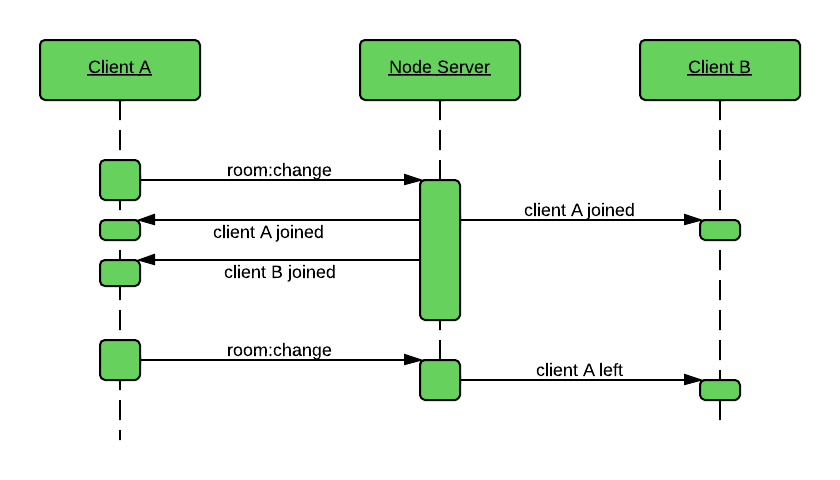
\includegraphics[width=15cm,keepaspectratio]{figures/join-seq.png}
\caption{Felhasználó belép a szobába}
\label{fig:joinseq}
\end{figure}

Az ábrán látszik, hogy szoba váltáskor a szerveroldal minden résztvevőjét a szobának (az új résztvevőt beleértve) értesít arról, hogy belépett, és az új résztvevőnek a létező socketek listáját is elküldi. Kilépéskor vagy diagram váltáskor is értesíti a klienseket. Így a kliensek nyilvántartást tudnak tartani a kapcsolódott többi kliensről. A \lstinline{client joined} és a \lstinline{client left} üzenetek esetében -- mivel az alkalmazás nem használ felhasználói fiókokat -- egy socket példány azonosítót is küld a kliensnek.

szinek mint userek
kep a jelolesrol  

162

Színek hogyan?